\documentclass[10pt,a4paper]{ULBreport}
\usepackage[utf8]{inputenc}
\sceau{pic/official_logos/sceauULB.png}
\graphicspath{ {./pic/} }
\usepackage{multirow}
\usepackage{listings}
\usepackage{color} 
\usepackage{setspace} 
\usepackage{amsmath}
\usepackage{hyperref}
\usepackage{pdfpages}
\usepackage{biblatex}
\usepackage{floatrow}
\usepackage{subcaption} 
\usepackage{siunitx}
\usepackage[many]{tcolorbox}
\usepackage{multirow}
\usepackage{listings}
\usepackage[dvipsnames]{xcolor}
\usepackage{fancyvrb}

\usepackage{xstring}
\usepackage{etoolbox}

% Colors

% BOXES FOR QUESTIONS

\newtcolorbox{Task}[2][]{
    fontupper=\bf,
    boxrule=1.5pt,
    colframe= black, % frame color
    fonttitle=\itshape,
    attach boxed title to top left={yshift=-0.3\baselineskip-0.4pt,xshift=2mm},
    title= #2,#1,
    enhanced,
    }

\begin{document} 


	\titleULB{
	title={Lab report},
    studies={IRELE},
    course ={Measurement and Data Driven Modelling},
    author={\textit{Authors :} \\ Arico Amaury \\ Colot Emmeran},
    date={\textbf{Academic year :} \\ 2024 - 2025},
    teacher={\textit{Professor : } \\ J. Lataire},
    logo={pic/official_logos/logos.jpg},
    manyAuthor
	}

%\listoftables % ToC for tables

%\listoffigures % ToC for figures

\setcounter{secnumdepth}{1}

\chapter{Lab 1}

\section{DFT}

\begin{Task}{Task 1.1.1.}
    Prove that
    \begin{equation*}
        \omega_k = \frac{2\pi}{T} k
    \end{equation*}
    where $T = nT_s$ is the window length.
\end{Task}

Starting from the general definition of the iDFT and the one in case of a discrete signal:

\begin{align*}
    x(n) = \frac{1}{N} \sum_{k=0}^{N-1} X(k) e^{\frac{j 2 \pi k n}{N}}\\
    x(n) = \frac{1}{N} \sum_{k=0}^{N-1} X(k) e^{j \omega_k n T_s}
\end{align*}

By simply comparing both equations, $\omega_k = \frac{2\pi}{n T_s} k$. Replacing the sampling period $T_s$ multiplied with the number of samples $n$ by the total sampling time, the result is obtained.

\begin{equation*}
    \omega_k = \frac{2\pi}{T} k
\end{equation*}

\begin{Task}{Task 1.1.2.}
    Prove that
    \begin{equation*}
        \omega_1 = \frac{2\pi}{T} = 2\pi \frac{f_s}{N}
    \end{equation*}
\end{Task}

The first equality is proven using the result of the previous task. By replacing $T$ the window length by $nT_s$ and then defining the sampling frequency $f_s = \frac{1}{T_s}$, the result is obtained.

\begin{Task}{Task 1.1.3.}
    Prove that
    \begin{equation*}
        X(N-k) = X(-k) = X^*(k)
    \end{equation*}
    \textit{Hint: Use $e^{j2\pi n} = 1$ for n $\in \mathbb{N}$ and $x(n) \in \mathbb{R}$.}
\end{Task}

By using the definition of the DFT, the following equation is obtained:

\begin{align*}
    X(k) = \sum_{n=0}^{N-1} x(n) e^{\frac{-j2\pi kn}{N}}\\
    X(N-k) = \sum_{n=0}^{N-1} x(n) e^{\frac{-j2\pi Nn}{N}-\frac{-j2\pi kn}{N}}\\
    X(N-k) = \sum_{n=0}^{N-1} x(n) e^{\frac{j2\pi kn}{N}}\\
\end{align*}

Where the last equality is obtained by removing the term $e^{-j2\pi n}$ which is equal to 1. By finally comparing the first and the third equation, one can see that only a minus sign is missing. Either $k$ is replaced by $-k$ giving:

\begin{equation*}
    X(N-k) = X(-k)
\end{equation*}

Either the conjugate of the whole equation is taken (needing the assumption that $x(n) \in \mathbb{R}$):

\begin{equation*}
    X(N-k) = X^*(k)
\end{equation*}

\section{DFT of a (co)sine}

\begin{Task}{Task 1.2.1. DFT of a 3 periods cosine}
    Generate a cosine sequence in Matlab with a randomly selected phase, and with a period that fits exactly 3 times in a data sequence of N = 1000 samples. Make a plot of the DFT of this sequence (amplitude and phase).
\end{Task}

\begin{figure}[H]
    \centering
    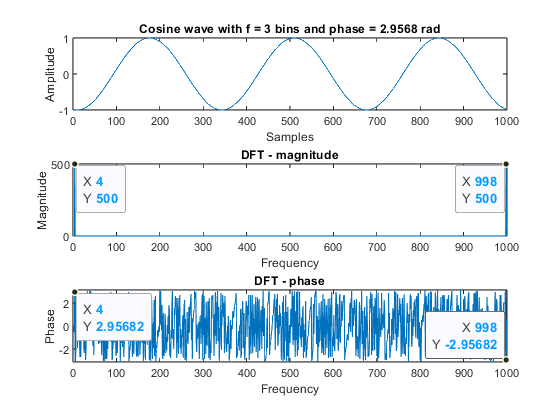
\includegraphics[width=1\textwidth]{part1/task1_2_1.png}
    \caption{DFT of a 3 periods cosine}
\end{figure}

Remarks: from the previous section, it is known that the DFT of a cosine at a frequency of 3 bins would create a peak at the third bin and one at the N - 3 bin as $X(N-k) = X^*(k)$. There is a shift of 1 bin as matlab indices starts at 1. concerning the phase plot, the phase at the third bin is indeed the one chosen randomly. The phases at the other bins are not relevant as the cosine is not present at these frequencies. The phase at the N - 3 bin is the opposite of the one at the third bin as $X(N-k) = X^*(k)$.

\begin{Task}{Task 1.2.2. Perfect reconstruction}
    From the DFT plot, check that the condition for perfect reconstruction is satisfied. Is there any leakage visible?\\
    \textit{Hint: use a logarithmic amplitude axis to distinguish small (but non-zero) values.}
\end{Task}

\begin{figure}[H]
    \centering
    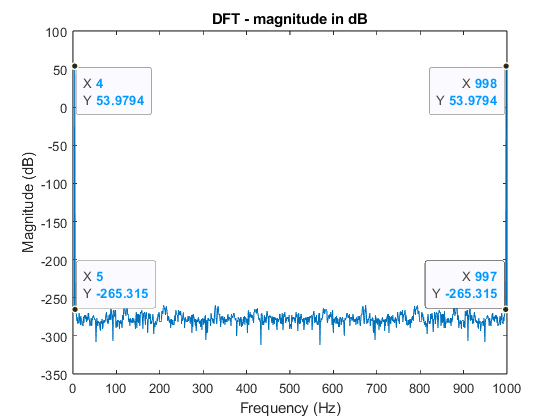
\includegraphics[width=1\textwidth]{part1/task1_2_2.png}
    \caption{Perfect reconstruction}
\end{figure}

There is a difference in amplitude of more than 300 dB between the excited bin and its neighbors. This shows that the condition for perfect reconstruction is satisfied.

\begin{Task}{Task 1.2.3. Intrpretation of the frequency axis}
    At which indices of the DFT do you obtain non-zero values? Explain. (Keep in mind that Matlab indices start at 1, not at 0.)
\end{Task}

As already discussed in task 1.2.1, the DFT of a cosine at a frequency of 3 bins would create a peak at the third bin and one at the N - 3 bin as $X(N-k) = X^*(k)$. There is a shift of 1 bin as matlab indices starts at 1. The other bins are (close to) zero as there is no excitations at these frequencies.

\begin{Task}{Task 1.2.4. Frequency axis in bins}
    Construct the frequency axis for the plots, expressed in bins.
\end{Task}

It is already done in the matlab script as the x-axis of the plots is expressed in "DFT samples number", which are in fact bins.

\begin{Task}{Task 1.2.5. Frequency axis in Hz}
    Consider that the sample frequency is fs = 100 Hz. Construct the frequency axis for the plots, expressed in Hz.\\
    \textit{(Hint: use the results from Task 1.1.1.)}
\end{Task}

\begin{figure}[H]
    \centering
    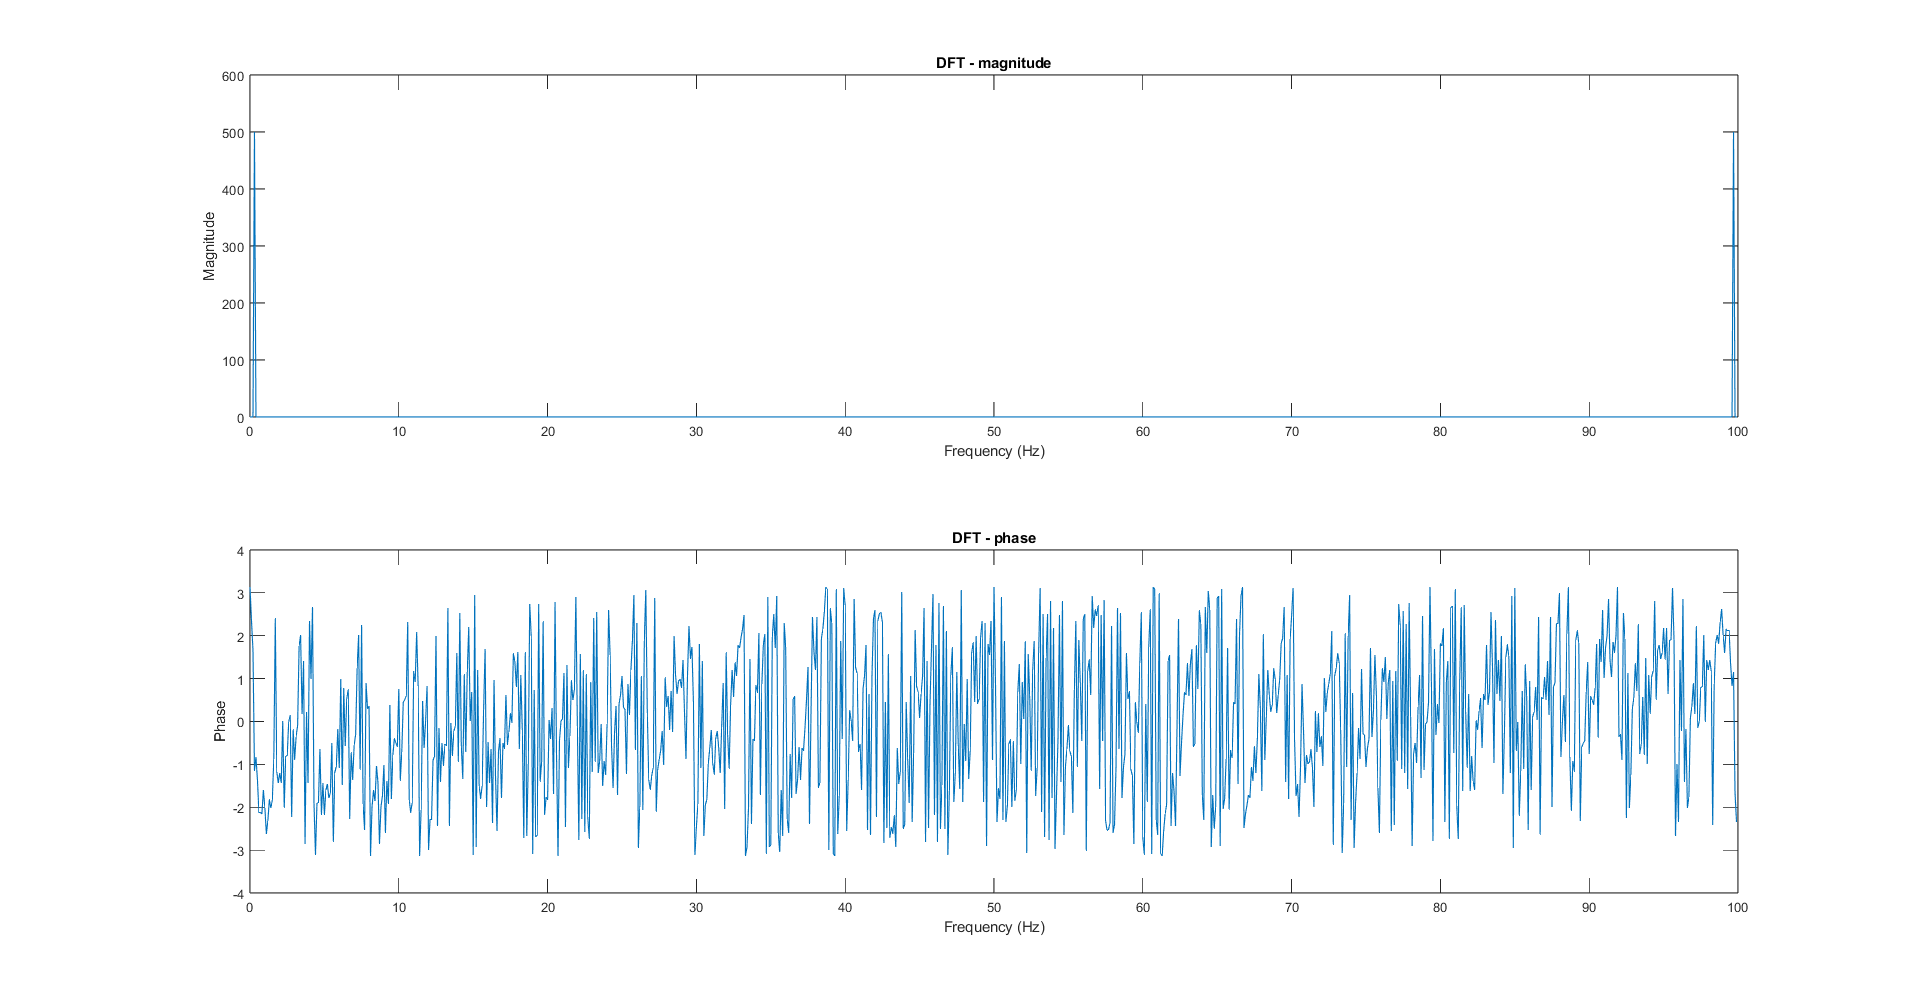
\includegraphics[width=1\textwidth]{part1/task1_2_5.png}
    \caption{Frequency axis in Hz}
\end{figure}

To change the frequency axis from bins to Hz, it was simply multiplied by $\omega_1 = \frac{f_s}{N}$.

\section{Time domain construction of a multisine}

\begin{Task}{Task 1.3.1. Time domain random phase multisine}
    Generate a multisine in the time domain, by implementing (1.6), with $N = 1000$ samples and $K = 10$ excited frequencies. Set the amplitudes $A_m = 1$, and choose the phases $\varphi_m$ randomly between $0$ and $2\pi$ (i.e. a random phase multisine). Check that this multisine satisfies the condition for perfect reconstruction by plotting its DFT. (Use a logarithmic amplitude axis). Include the frequency axis, expressed in bin.
\end{Task}

\begin{figure}[H]
    \centering
    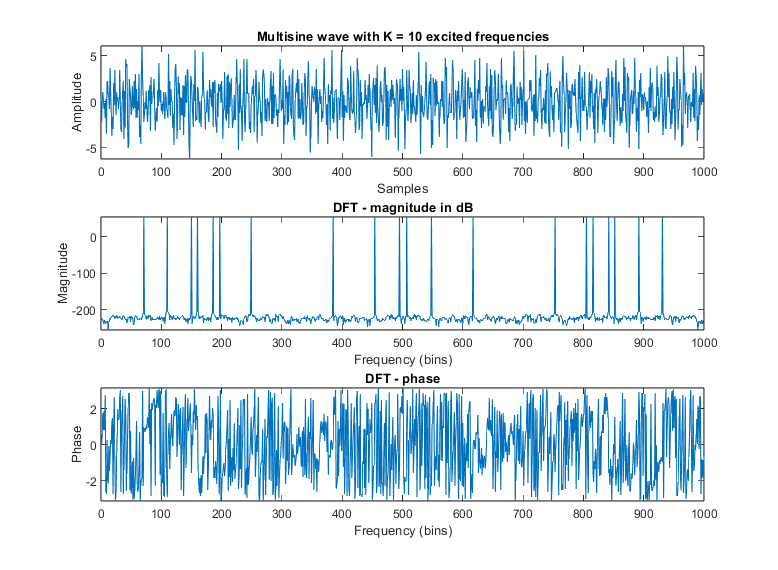
\includegraphics[width=1\textwidth]{part1/task1_3_1.png}
    \caption{Time domain random phase multisine}
\end{figure}

The condition for perfect reconstruction is satisfied as the difference in amplitude between the excited bins and their neighbors is more than 250 dB.

\begin{Task}{Task 1.3.2. Frequency axis in Hz}
    For the multisine generated in Task 1.3.1, consider that the sampling frequency is $f_s = 100 Hz$. Include the frequency axis expressed in Hz in the DFT plot, and the time axis expressed in seconds for the time domain plot.
\end{Task}

\begin{figure}[H]
    \centering
    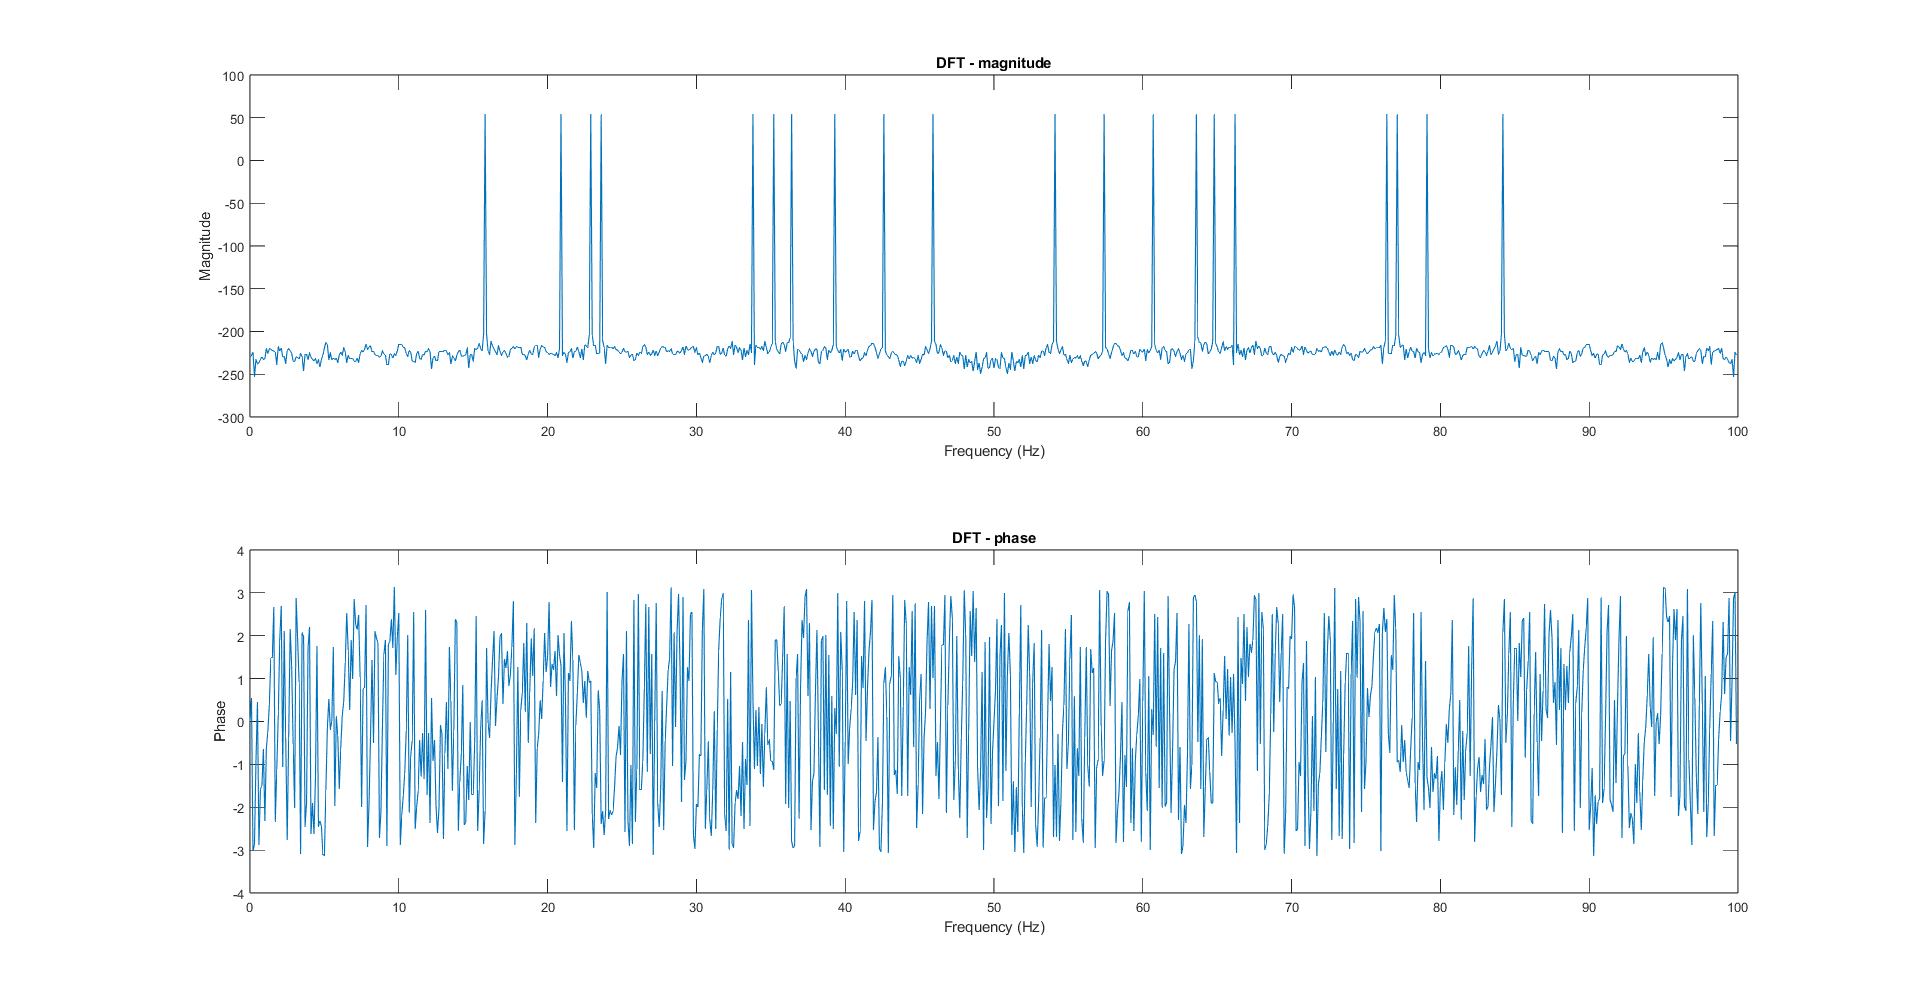
\includegraphics[width=1\textwidth]{part1/task1_3_2.png}
    \caption{Frequency axis in Hz}
\end{figure}

As in task 1.2.5, the frequency axis was converted from bins to Hz by multiplying it by $\omega_1 = \frac{f_s}{N}$.

\begin{Task}{Task 1.3.3. Excite specific frequencies}
    Generate a random phase multisine with a sampling frequency of $200 Hz$, with excited frequencies
    \begin{equation*}
        [4, 8, 12, 16, 20, 24] Hz
    \end{equation*}
    Plot the time and frequency domain results, with appropriate axes.
\end{Task}

\begin{figure}[H]
    \centering
    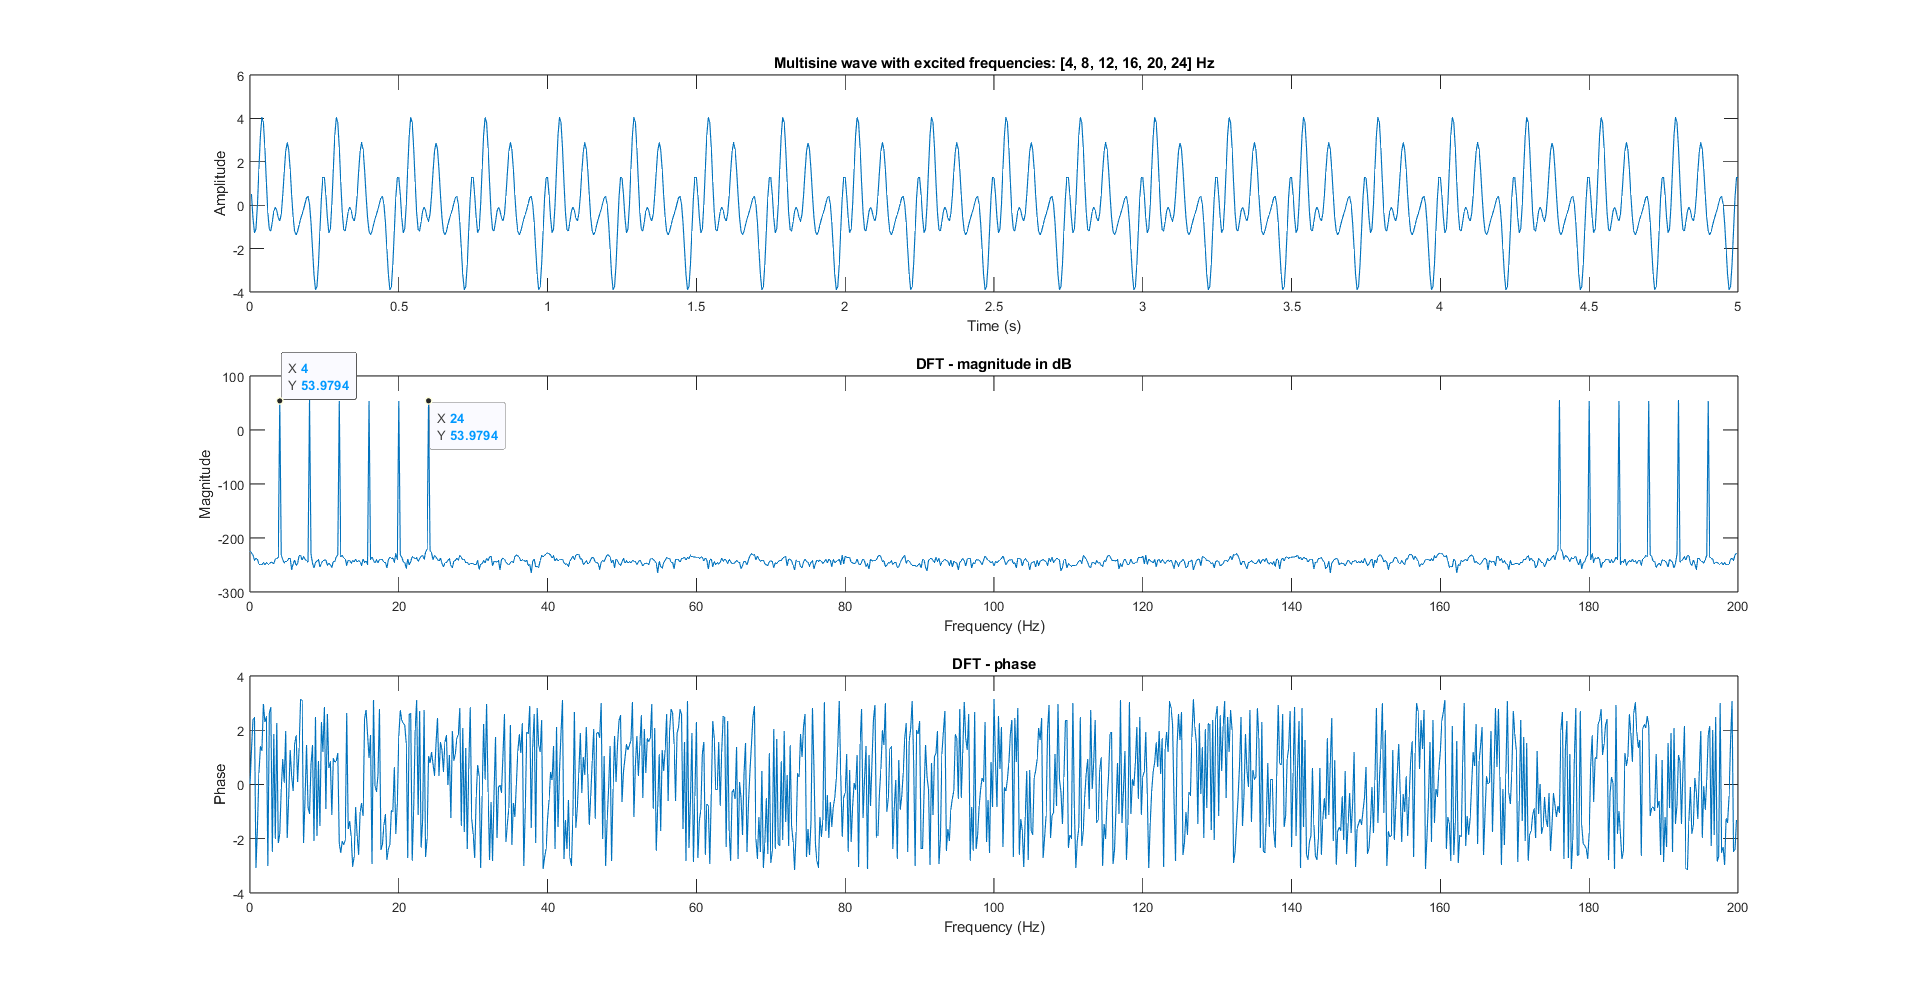
\includegraphics[width=1\textwidth]{part1/task1_3_3.png}
    \caption{Excite specific frequencies}
\end{figure}

\section{Frequency domain construction of a multisine}

\begin{Task}{Task 1.4.1. Trick for frequency domain multisine construction}
    Consider the vector $\tilde{X}(k)$, such that
    \begin{align*}
        \tilde{X}(k) = A_ke^{j\varphi _k} && \text{for} 1 \leq k \leq K\\
        \tilde{X}(k) = 0 && \text{otherwise}
    \end{align*}
    Prove that
    \begin{equation*}
        x(n) = N \Re \left\{\text{iDFT}(\tilde{X}(k))\right\} = \sum_{k = 1}^{K} A_k \cos(\frac{2\pi k}{N} + \varphi_k)
    \end{equation*}
    Where $\Re$ denotes the real part.\\
    \textit{Hint: use the definition of the iDFT}
\end{Task}

Starting from the definition of the iDFT:

\begin{align*}
    x(n) &= \frac{1}{N} \sum_{k=0}^{N-1} X(k) e^{\frac{j 2 \pi k n}{N}}\\
    &= \frac{1}{N} \sum_{k = 1}^{K} A_k e^{j \varphi_k} e^{\frac{j 2 \pi k n}{N}}\\
    &= \frac{1}{N} \sum_{k = 1}^{K} A_k e^{\frac{2\pi k}{N} + \varphi_k}
\end{align*}

By then taking the real part of $x(n)$ and multiplying it by $N$:

\begin{align*}
    x(n) &= \frac{N}{N} \sum_{k = 1}^{K} A_k \Re \left(e^{\frac{2\pi k}{N} + \varphi_k}\right)\\
    &= \sum_{k = 1}^{K} A_k \cos(\frac{2\pi k}{N} + \varphi_k)
\end{align*}

\begin{Task}{Task 1.4.2. Frequency domain multisine}
    Use the frequency domain approach to construct a random phase multisine, by using the trick from Task 1.4.1. Let $N = 1000$, and excite the first $30$ bins. Make time and frequency domain plots (frequency axis expressed in bins).
\end{Task}

\begin{figure}[H]
    \centering
    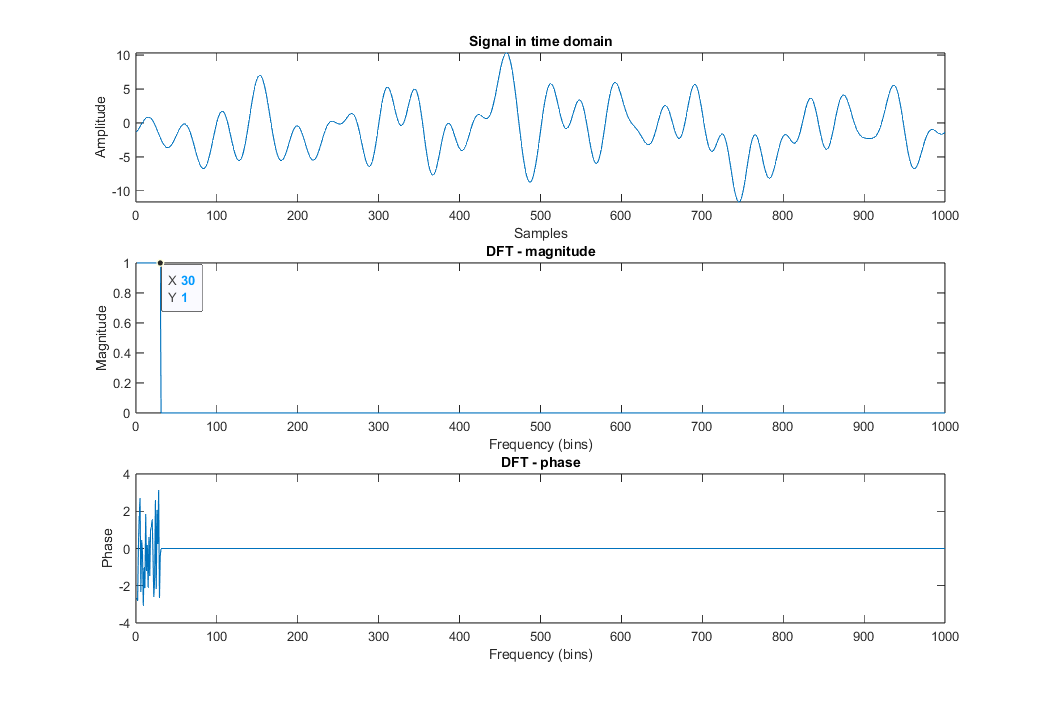
\includegraphics[width=1\textwidth]{part1/task1_4_2.png}
    \caption{Frequency domain multisine}
\end{figure}

\begin{Task}{Task 1.4.3. Specified excited frequency band and frequency resolution}
    Construct a random phase multisine in the frequency domain, which excites the frequency band [5, 15] Hz at 30 equidistantly spaced frequencies. Choose an appropriate sampling frequency. Make time domain and frequency domain plots (time axis in seconds, frequency axis in Hz). How long is one period of this multisine (expressed in seconds)?
\end{Task}

A frequency band of 10 Hz with 30 equidistantly spaced frequencies means that a bin must be equal to $1/3 Hz$ (or a divider of it). Using the formula of $\Delta_f = \frac{f_s}{N}$ (where $\Delta_f$ is the frequency resolution) and using a sampling frequency $f_s$ larger than twice the maximum signal frequency:
\begin{equation*}
    f_s = 50 Hz \quad\quad\quad\quad N = 3 f_s = 150
\end{equation*}

\begin{figure}[H]
    \centering
    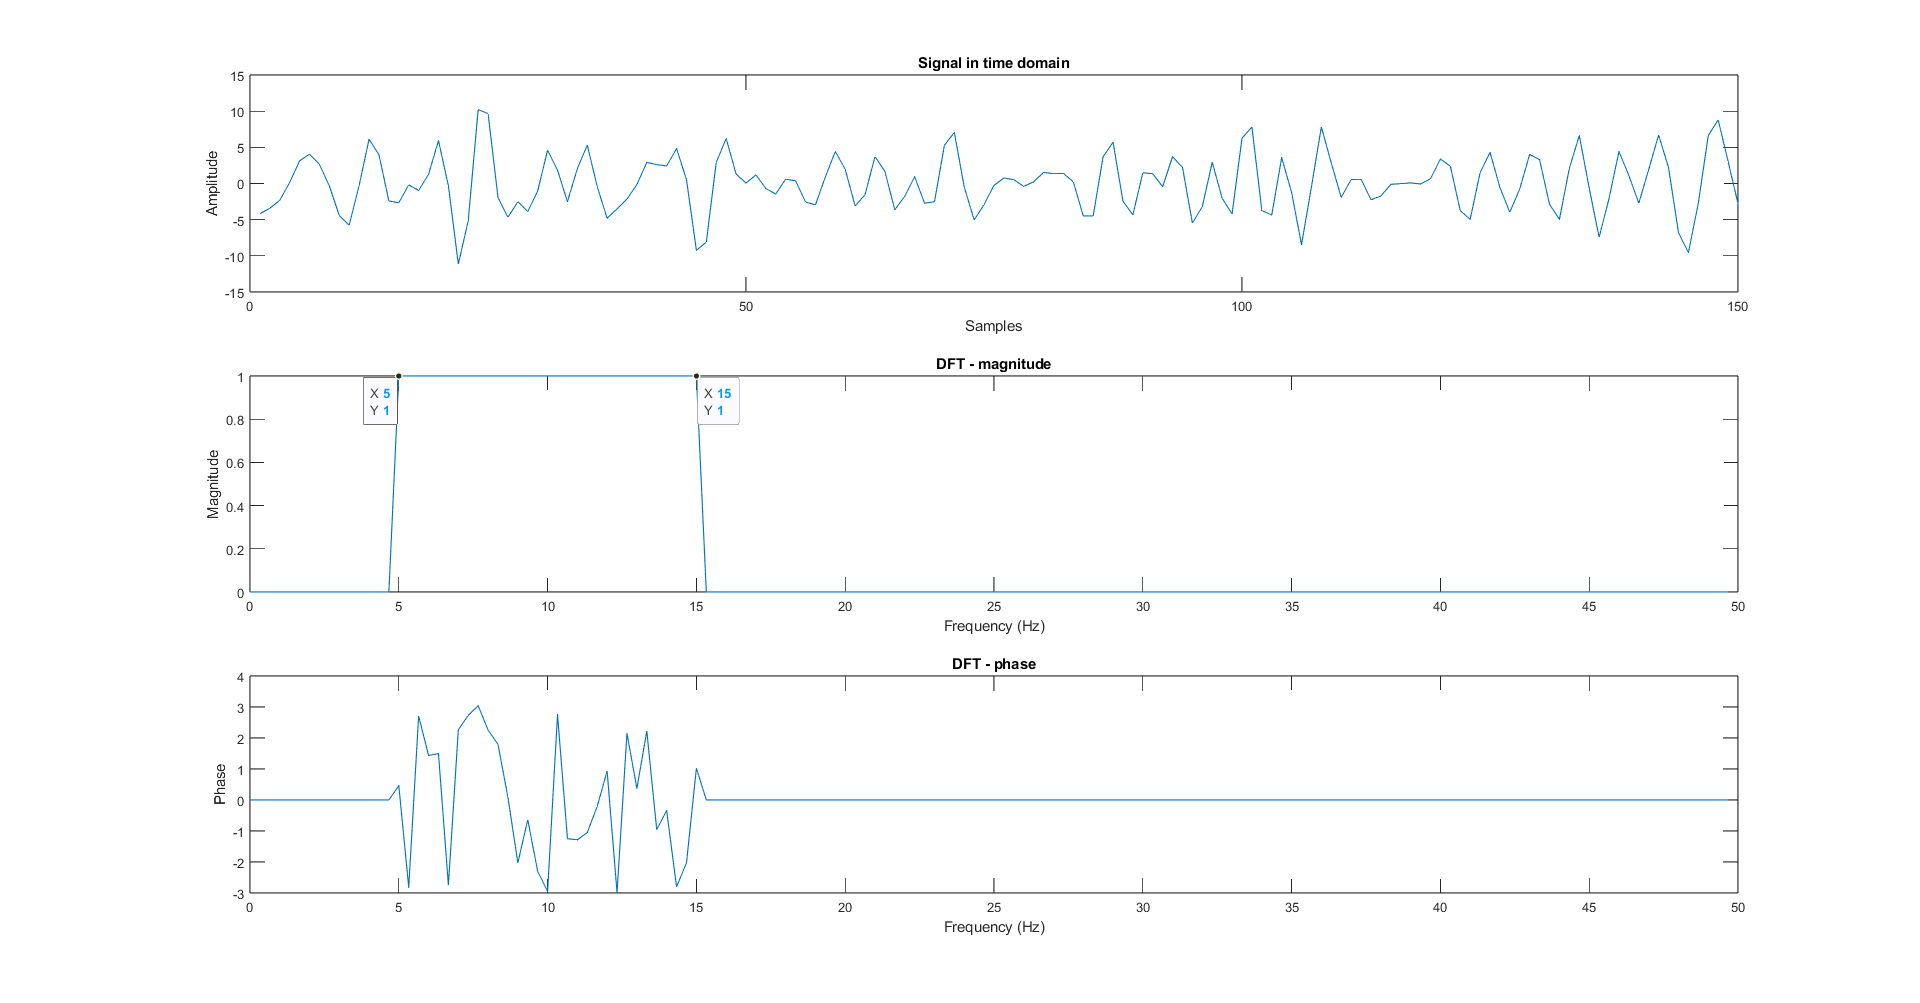
\includegraphics[width=1\textwidth]{part1/task1_4_3.png}
    \caption{Specified excited frequency band and frequency resolution}
\end{figure}

Because it was built with the perfect reconstruction condition, the period of the multisine is equal to the period of a sine at the frequency resolution, which is $1/3 Hz$ so the period is $3$ seconds.

\section{Influence of the phase of the multisine}

\begin{Task}{Task 1.5.1. Crest Factor}
    Construct a multisine, with N = 500, with the first K = 60 bins excited, and with the following phases:
    \begin{itemize}
        \item random phase: chosen randomly in $[0, 2\pi]$ (uniform distribution)
        \item Schroeder phase: $\varphi_k = \frac{m(m+1)\pi}{K}$
        \item Linear phase: $\varphi_m = m\pi$
    \end{itemize}
    Make time and frequency domain plots (in samples and bins), and compute the Crest Factors. Describe, qualitatively, the relationship between the time domain plot and the crest factor. What is the advantage of a low/high crest factor?
\end{Task}

\begin{figure}[H]
    \centering
    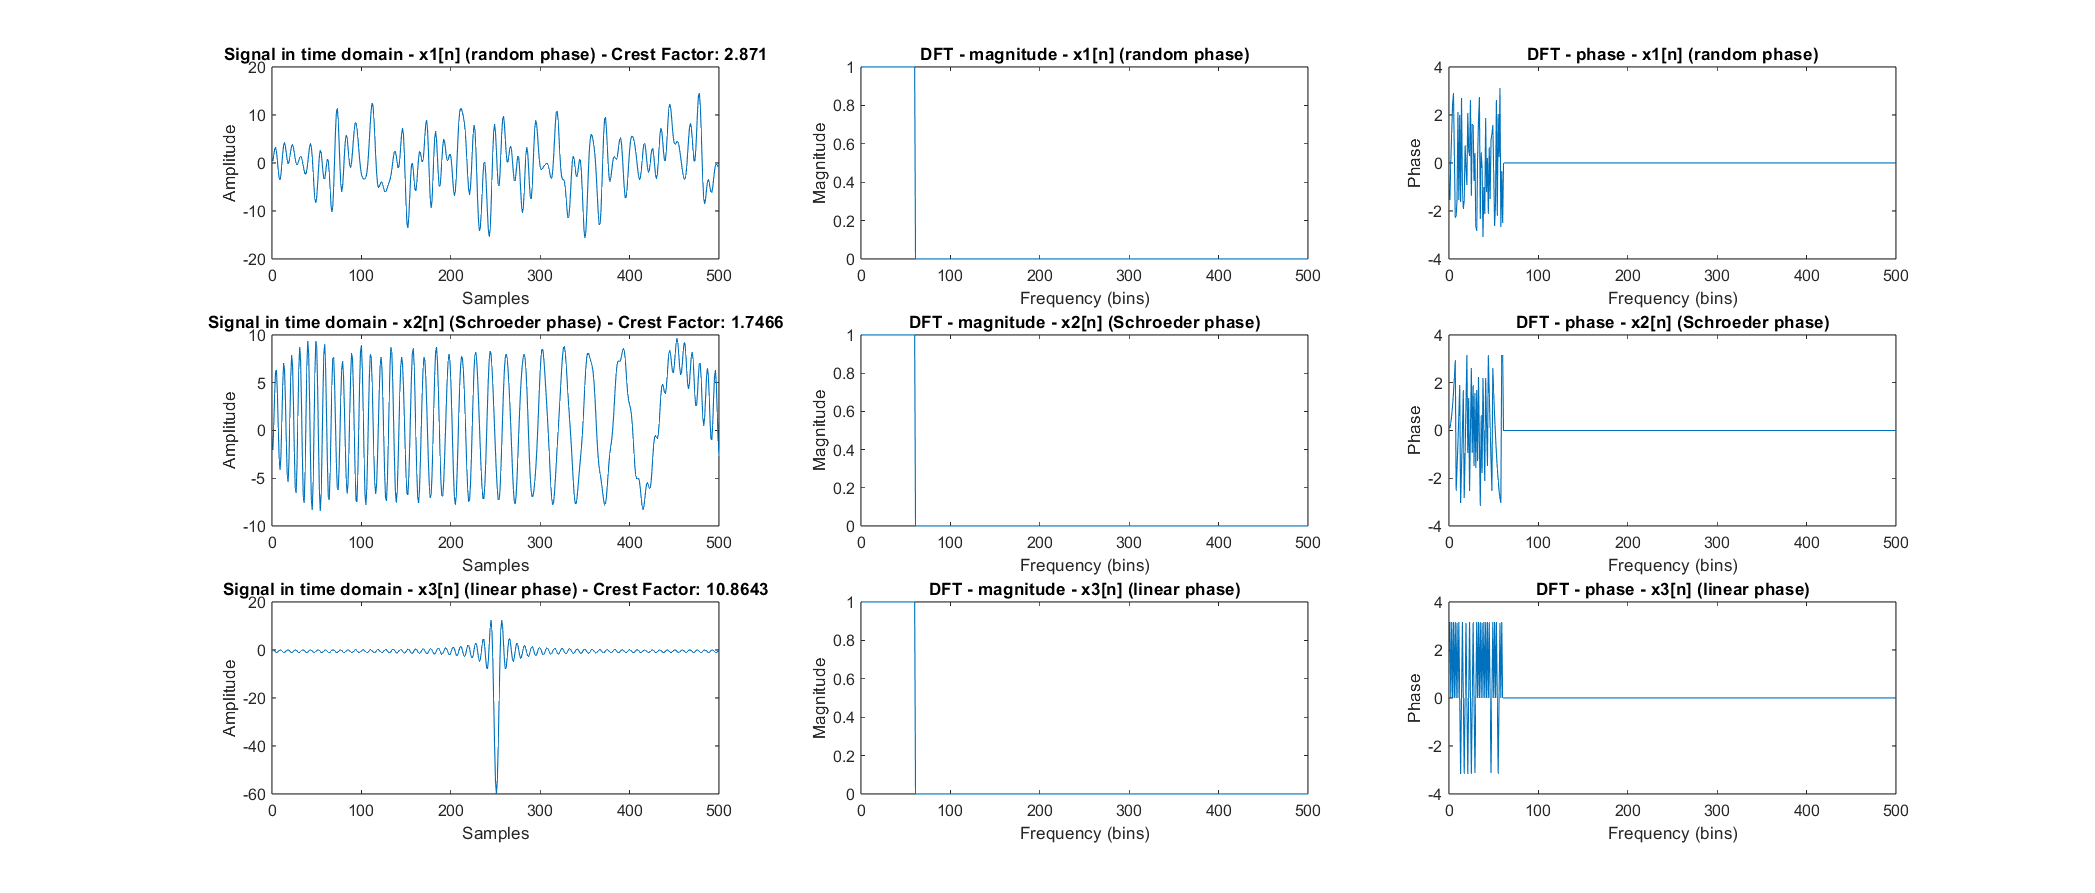
\includegraphics[width=1\textwidth]{part1/task1_5_1.png}
    \caption{Crest Factor}
\end{figure}

Based on the figure, it is quite clear that a larger Crest Factor corresponds to a signal that has peaks of larger amplitude ($\max |x_3| \approx 6 \times \max |x_2|$). This is easily understandable as the Crest Factor is defined as the ratio between the peak value and the RMS value of the signal. The advantage of a low Crest Factor is that the signal has no big peaks, which could damage an unprotected electronic system receiving it.

\section{Random noise signals}

\begin{Task}{Task 1.6.1. White Gaussian random noise}
    Generate a normally distributed (Gaussian), random, white noise sequence of N = 1000 samples, by using the Matlab function randn. Make time and frequency domain plots (axes in samples and bins). Observe that all the bins are excited, with random amplitudes and phases.
\end{Task}

\begin{figure}[H]
    \centering
    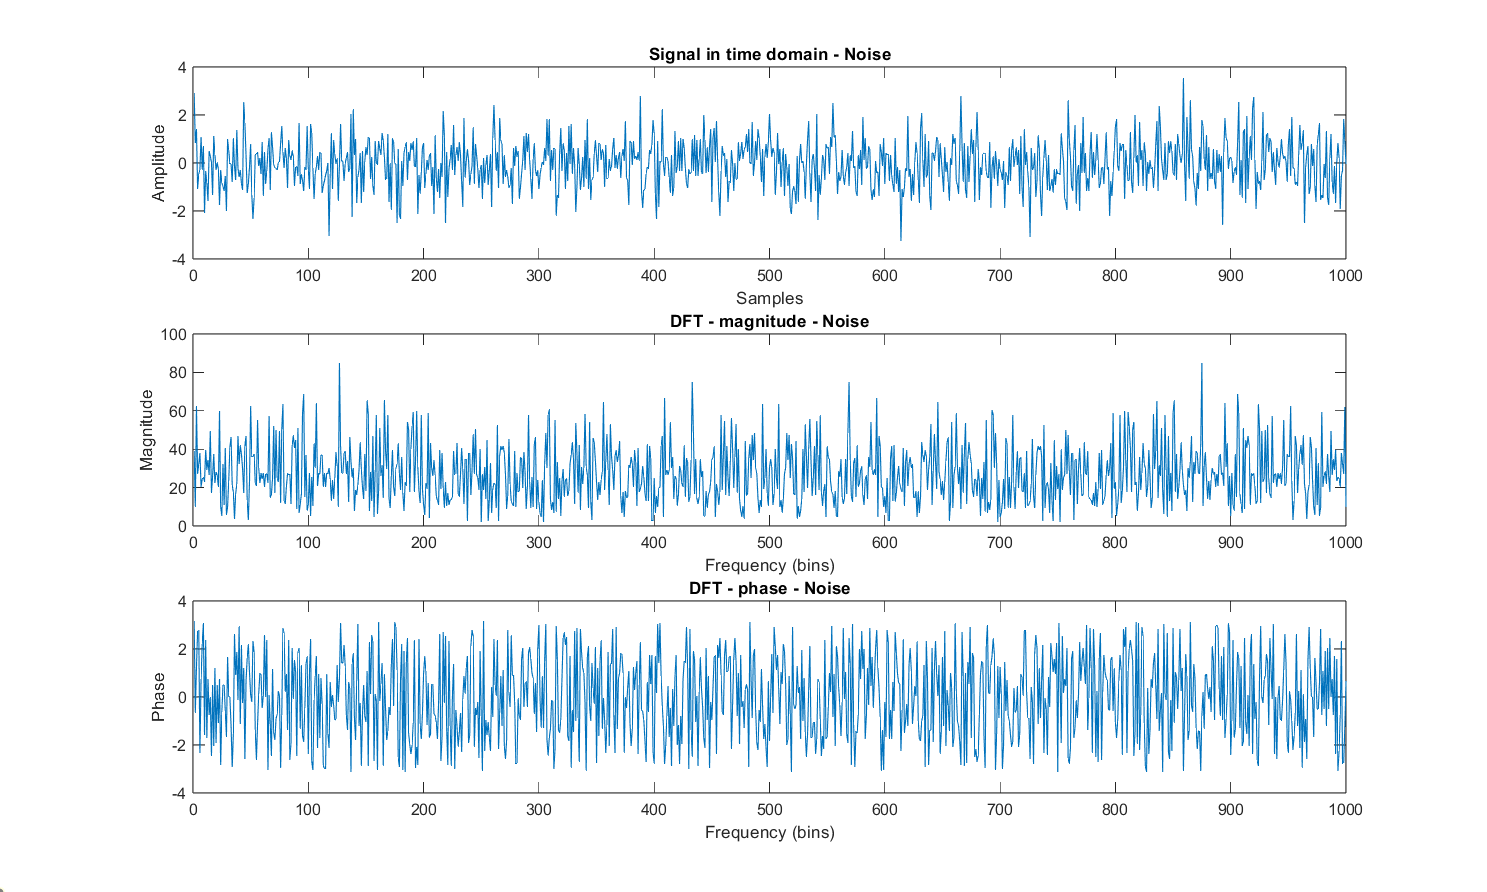
\includegraphics[width=1\textwidth]{part1/task1_6_1.png}
    \caption{White Gaussian random noise}
\end{figure}

\begin{Task}{Task 1.6.2. Filtered random noise}
    Generate a filtered random noise sequence with N = 1000, sampling frequency 100 Hz, from a Gaussian white noise sequence (use randn). Do this by using the function cheby1 to create a lowpass digital Chebyshev filter of order 5, ripple 2 dB, and such that the passband edge lies at 5 Hz. Filter the sequence by using the function filter. Make time and frequency domain plots (axes in seconds and Hz), and check that the excited frequency band is as expected. What do you observe in the stop-band of the filter? Is it equal to 0? Explain.
\end{Task}

\begin{figure}[H]
    \centering
    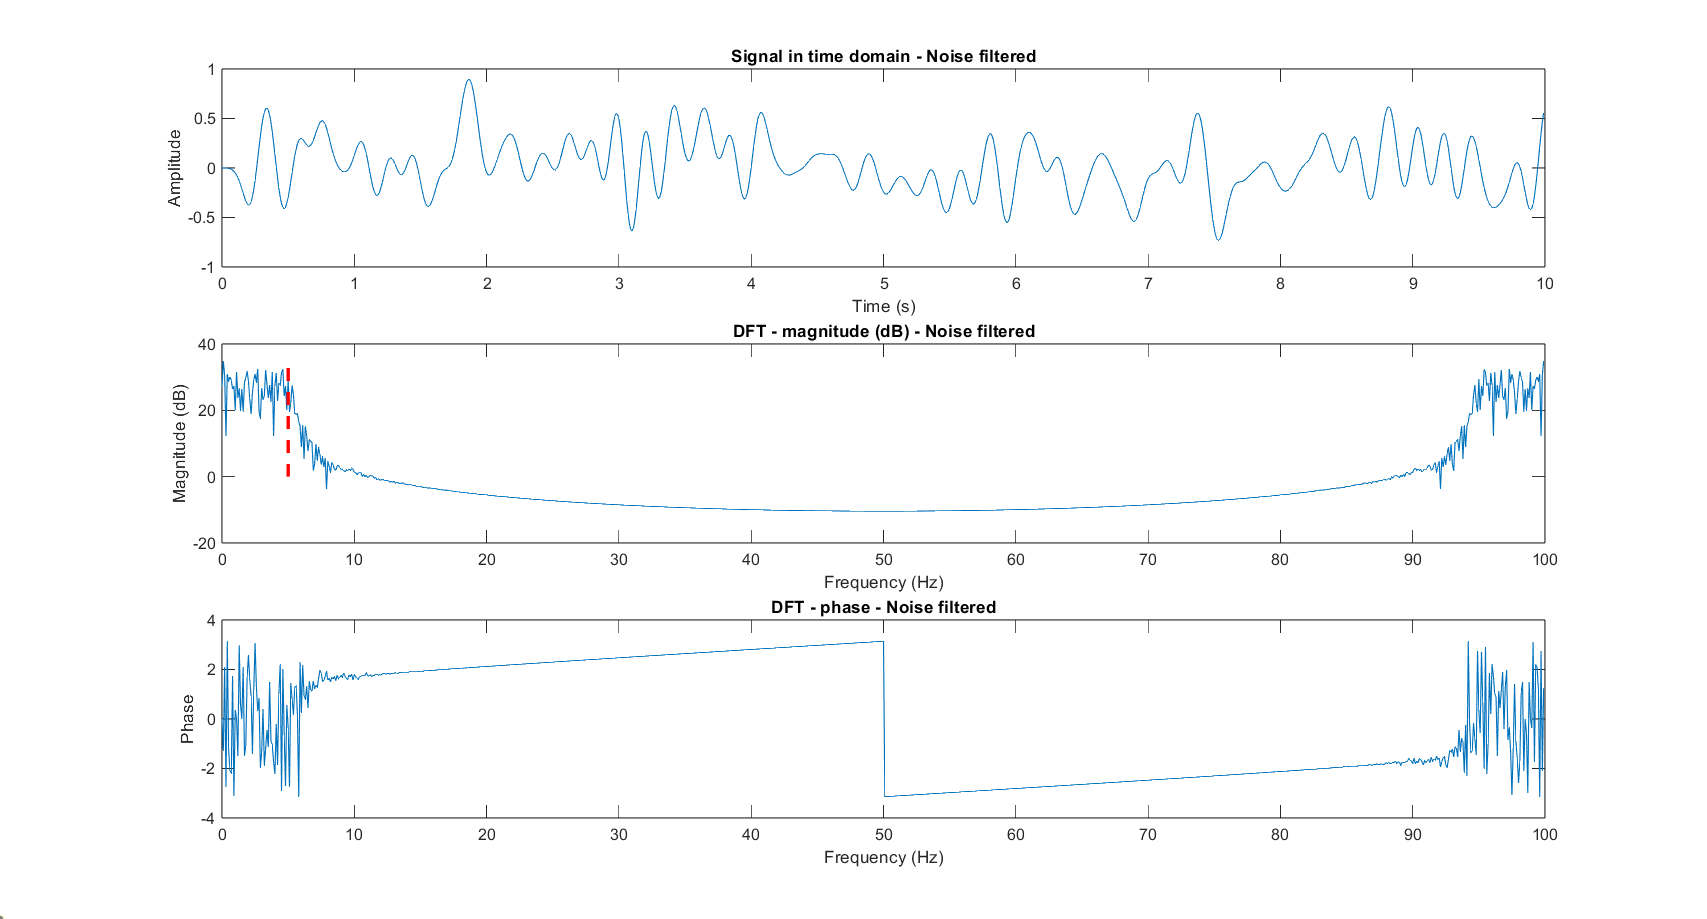
\includegraphics[width=1\textwidth]{part1/task1_6_2.png}
    \caption{Filtered random noise}
\end{figure}

The excited frequency band is indeed reduced to 5 Hz as expected. In the stop-band of the filter, the amplitude is not equal to 0. This is due to the fact that the filter is not an ideal filter, and thus does not completely remove the frequencies above 5 Hz. The amplitude after $10 Hz$ is already reduced by $30 dB$ and the increase for higher bins is due to the symmetry of the DFT proved in task 1.1.3.

\begin{Task}{Task 1.6.3. Periodic band-limited random noise}
    Generate a Gaussian random noise sequence (use randn), with N = 1000 and sampling frequency 100 Hz. Compute the DFT, and set the DFT at all frequencies beyond 5 Hz to zero:
    \begin{align*}
        \tilde{X}(k) = 0 && \text{for } \omega_k \geq 10\pi \text{ rad/s}\\
        \tilde{X}(k) = X(k) && \text{otherwise}
    \end{align*}
    and use the expression
    \begin{equation*}
        x(n) = 2 \Re \left\{\text{iDFT}(\tilde{X}(k))\right\}
    \end{equation*}
    to obtain the time sequence. Make time and frequency domain plots (axes in seconds and Hz).\\
    If you repeat this time domain sequence x(n) (by putting multiple copies of the sequence after each other), and computing the DFT of the result, no leakage should occur. Check this, and explain why this is the case.
\end{Task}

\begin{figure}[H]
    \centering
    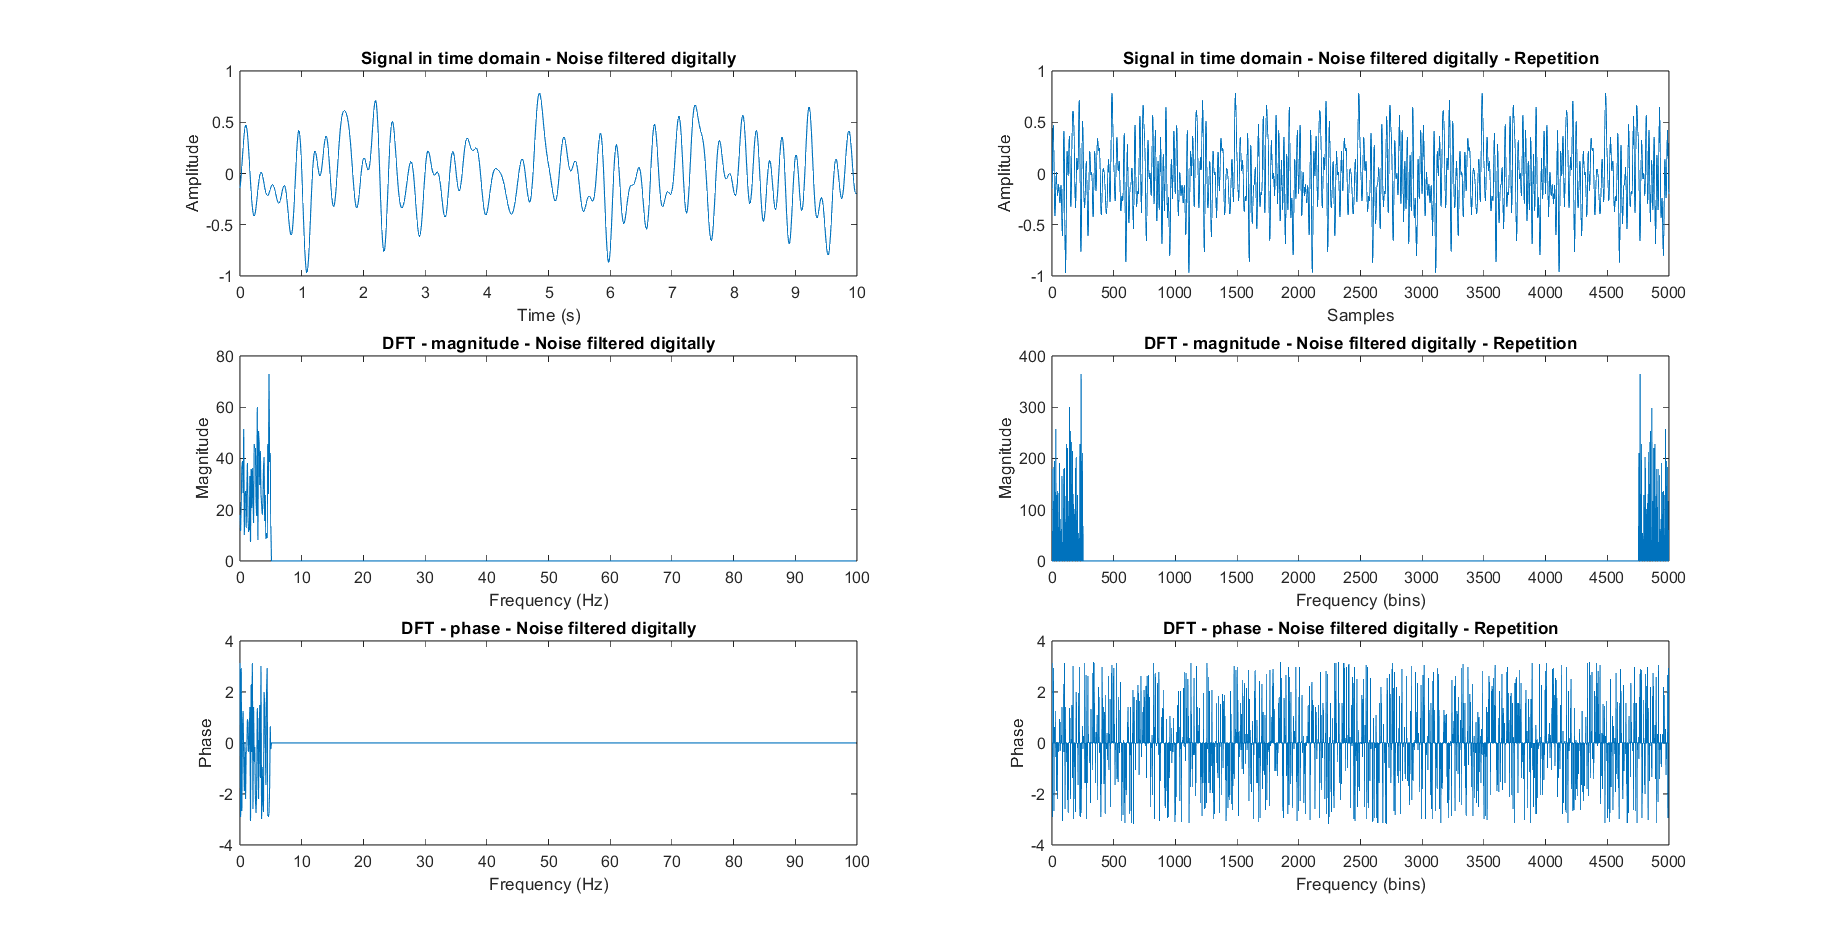
\includegraphics[width=1\textwidth]{part1/task1_6_3.png}
    \caption{Periodic band-limited random noise}
\end{figure}

There is no leakage when repeating the \textbf{idft} of the filtered noise as the condition on perfect reconstruction is fulfilled. As the signal that is repeated is built from the frequential domain, it will have an integer number of periods in the time domain, and thus when replicated no leakage will occur as it will still have an integer number of periods inside the window of the \textbf{dft}.

\section{Set the Root-Mean-Square of the signal}

\begin{Task}{Task 1.7.1. RMS value}
    Set the RMS value of your favourite signal from the previous tasks to $RMS_{des} = 3$, as follows:
    \begin{equation*}
        x_{des}(n) = x(n)\frac{RMS_{des}}{RMS(x)}
    \end{equation*}
    Prove that thr RMS of $x_{des}(n)$ is indeed $RMS_{des}$.
\end{Task}

\begin{figure}[H]
    \centering
    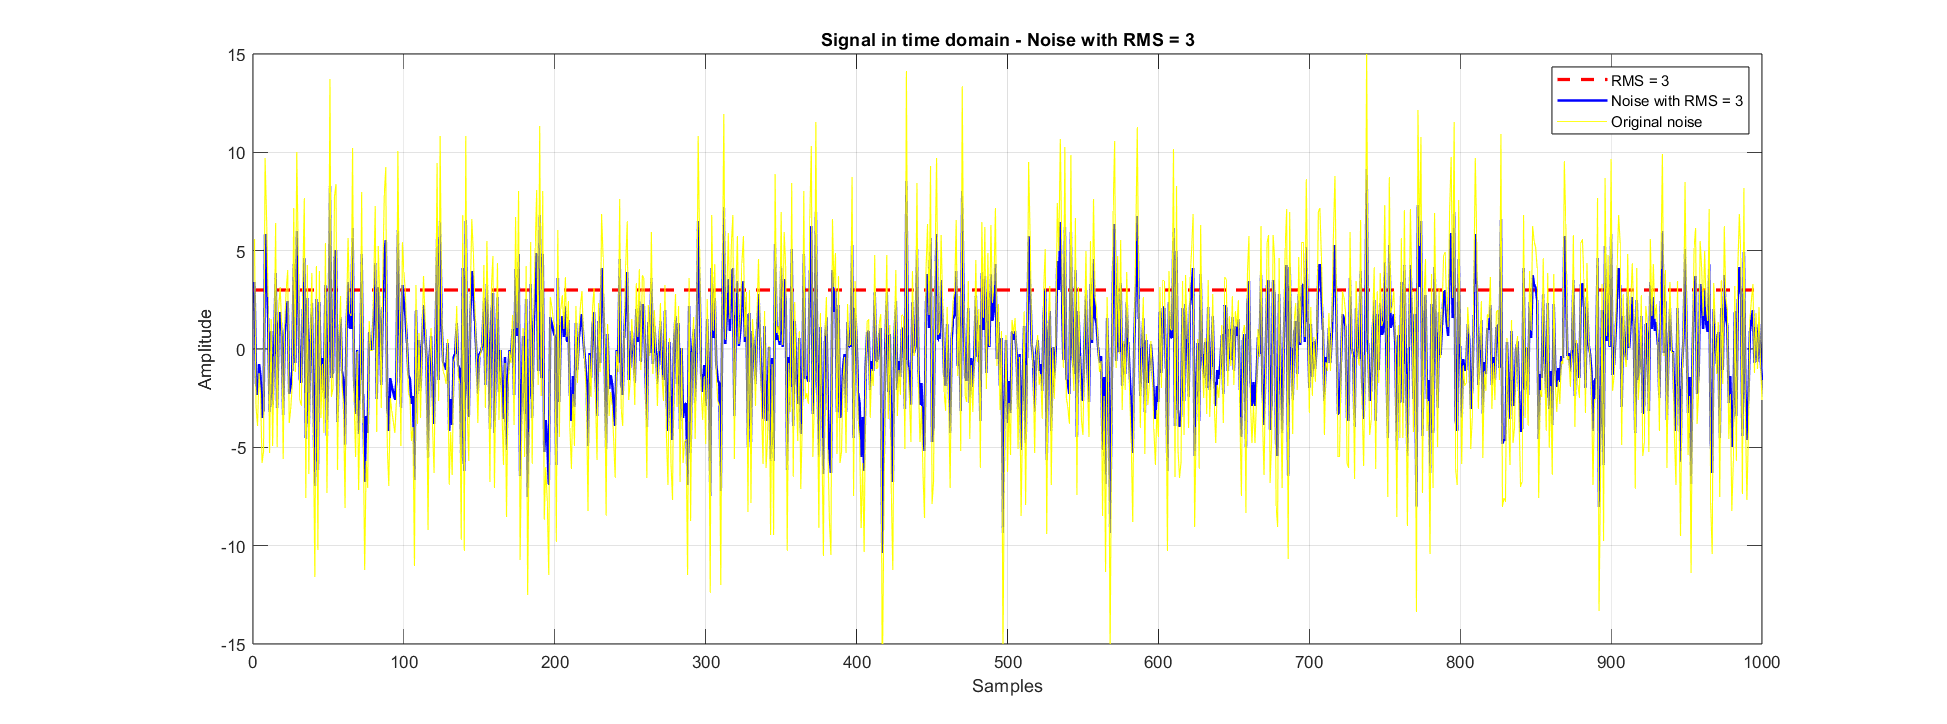
\includegraphics[width=1\textwidth]{part1/task1_7_1.png}
    \caption{RMS value}
\end{figure}

Note that the title of the plot contains the RMS value of the modified signal and it indeed reaches $3$.

\setcounter{secnumdepth}{1}

\chapter{Lab 2}



\setcounter{secnumdepth}{1}

\chapter{Lab 3}


\begin{Task}{Question 3.1. Length data records}
    Note that this algorithm works faster when the length of the data records N is a power of 2. Do you know why?
\end{Task}

To implement numerically the FFT, the DFT algorithm is used. It works by dividing the input signal into two parts, each of which is transformed separately, and then the results are combined and this is done recursively. It means that a number of samples that is a power of 2 will be perfectly divided at each step, leading to a faster computation.

\begin{Task}{Question 3.2. Trigger signal}
    What is the purpose of a trigger signal? A number of processing methods were discussed in the theory to improve the SNR of the FRF by averaging of measurements. Which methods require a trigger signal to operate properly? Explain what happens if the trigger is absent while needed.
\end{Task}

For the averaging in the time domain and the averaging in the DFT spectra, the input and output signals need to be identical:
\begin{align*}
    H_{\text{time}}(j\omega_k) = \frac{\textbf{DFT}\left(\frac{1}{M}\sum_{i=1}^{M}y_i(n)\right)}{\textbf{DFT}\left(\frac{1}{M}\sum_{i=1}^{M}u_i(n)\right)}\\
    H_{\text{DFT}}(j\omega_k) = \frac{\frac{1}{M}\sum_{i=1}^{M}\textbf{DFT}\left(y_i(n)\right)}{\frac{1}{M}\sum_{i=1}^{M}\textbf{DFT}\left(u_i(n)\right)}
\end{align*}

For the measurements to be identical between two repetitions (except for the noise of course), they should always start at the same point in the period of the excitation and this is the purpose of the trigger signal.

\begin{Task}{Question 3.3. Frequency domain multisine}
    In your report, show the Matlab code you used to construct the multisine signal (with random or Schroeder phase) in the frequency domain. Make sure that the code is sufficiently commented to improve its readability.
\end{Task}

\begin{lstlisting}[language=Matlab]
fs = 16000; % Sampling frequency
excFreq = [4 1000]; % Excited frequencies in Hz
rmsVal = 0.5; % RMS value
N = 4000; % Number of samples

freqAxis = (0:N-1)*fs/N; % Frequency axis in Hz

K = (excFreq(2) - excFreq(1))*N/fs; % Number of excited frequencies

signalFreq = zeros(1, N);

for i = 1:length(freqAxis)
    if (freqAxis(i) >= excFreq(1) && freqAxis(i) <= excFreq(2))
        schroederPhase = (i*(i+1)*pi)/(K);
        signalFreq(i) = exp(1j*schroederPhase);
    end
end

signalTime = N*real(ifft(signalFreq)); % Generate the signal
signalTime = signalTime*rmsVal/rms(signalTime); % Normalize the signal
\end{lstlisting}


\begin{Task}{Question 3.4. Averaging the measurements}
    Which averaging techniques are applicable to which excitation signals? Explain.
\end{Task}

\huge{TODO}
\normalsize

\begin{Task}{Question 3.5. Plots}
    Provide relevant plots of the estimated FRF, obtained with the different methods, with the different exciation signals and with a different number of averaged records.
\end{Task}

\huge{TODO}
\normalsize

\begin{Task}{Question 3.6. Impact of repetition number}
    Determine the effect of the number of averaged records on the variability of the averaged result. Compare the standard deviation.
\end{Task}

\huge{TODO}
\normalsize

\begin{Task}{Question 3.7. Discussion}
    Discuss the differences and explain according to you, which will deliver the best result. Discuss the pros and cons of each excitation signal.
\end{Task}

\huge{TODO}
\normalsize

\setcounter{secnumdepth}{1}

\chapter{Lab 4}

\begin{Task}{Question 4.1. harmonic and intermodulation distortion}
    Consider a static nonlinear system whose response is given by:\\
    \begin{equation}
        y(t) = u(t) - \frac{1}{2}u^3(t) - \frac{1}{4} u^4(t)
    \end{equation}
    At which frequencies will energy appear at the output when the input is excited by the sum of 2 sinewaves, one at frequency 4Hz and one at frequency 11Hz?    
\end{Task}

using matlab, each excited frequency has been plotted on figure \ref{fig:distortionEx}. The different amplitudes are not correct, they simply give the order of magnitude of each frequency component. A more exact simulation with the fft of the output signal is shown in figure \ref{fig:distortionExExact}.

\begin{figure}[H]
    \centering
    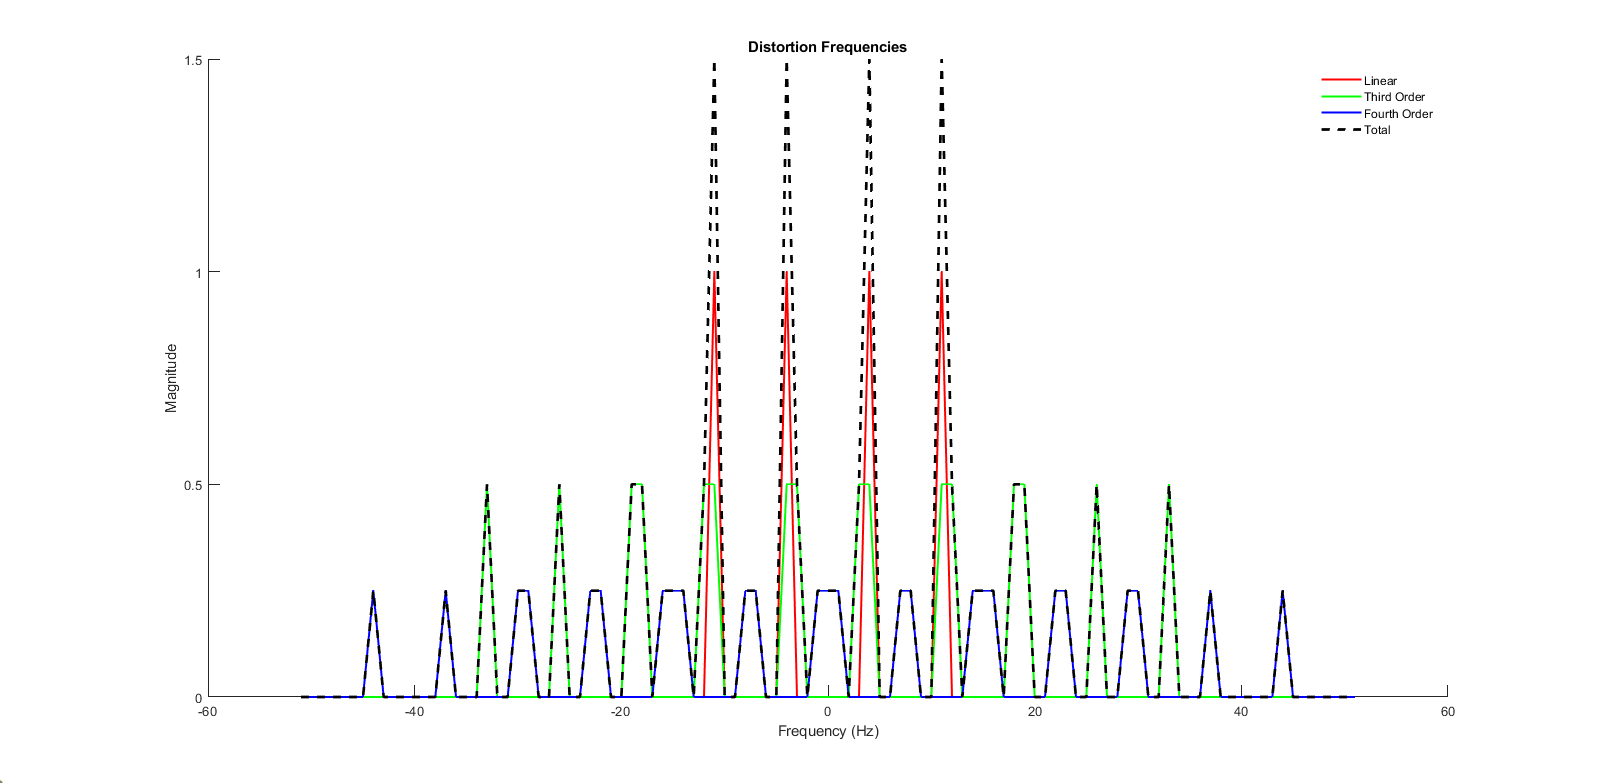
\includegraphics[width=0.8\textwidth]{part4/distortionEx.png}
    \caption{Excited frequencies - Approximation}
    \label{fig:distortionEx}
\end{figure}

\begin{figure}[H]
    \centering
    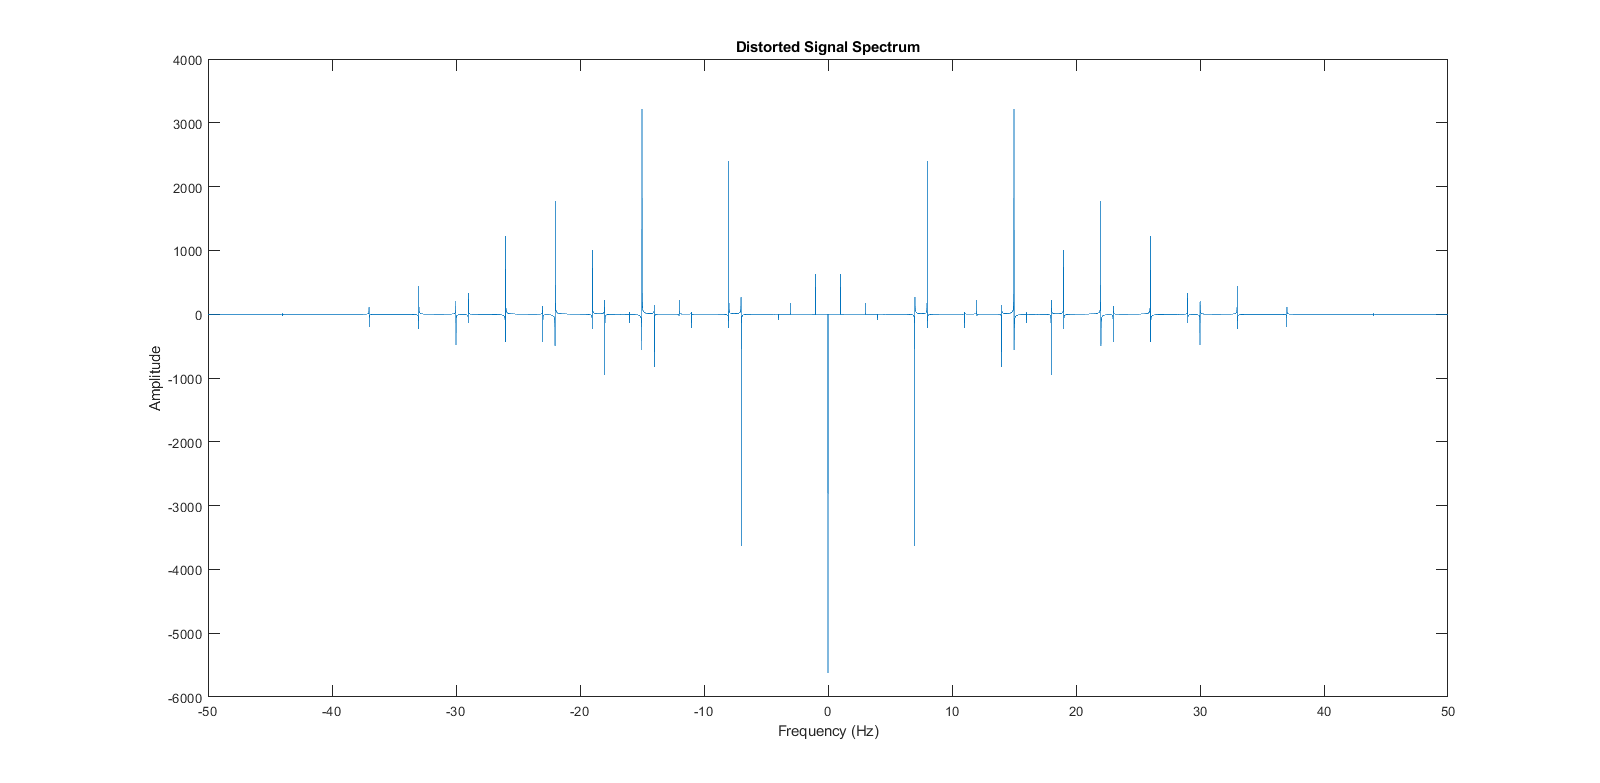
\includegraphics[width=0.8\textwidth]{part4/distortionExExact.png}
    \caption{Excited frequencies - Exact}
    \label{fig:distortionExExact}
\end{figure}

\begin{Task}{Question 4.2.}
    Design an excitation sinewave with a frequency of $100$ Hz and an amplitude of $1$ V. Plot the input signal and the output signal of the DUT in the frequency domain. What do you observe? Give a list of all possible solutions to get rid of this behaviour. Design experiments to show that the proposed solutions do indeed work.
\end{Task}

\begin{Task}{Question 4.3.}
    Change the excitation frequency to a frequency in the neighborhood of 100 Hz in order to solve the problem in the previous step. Use 10 different amplitudes that are spaced logarithmicaly from 100 mV to 1.1 V [logspace command in MATLAB]). Plot the DFT of the output for each amplitude. What are the frequencies at which you expect distortion to appear? Are they all present in reality? Explain.
\end{Task}

\begin{Task}{Question 4.4.}
    Plot the measurements from the previous question on an input power – output power plot. Do you see compression or expansion? From this plot, estimate the 1 dB compression or expansion point. Generate a single sine wave with the corresponding input amplitude to see how accurate your estimate is.
\end{Task}



%\printglossary

%\printglossary[type=\acronymtype]

%Bibliography
%\nocite{*}
%\printbibliography[type=article,title=Articles]

\end{document}	
